\chapter{\leavevmode\newline The Large Hadron Collider}
\label{chap:chapter_2}

The Large Hadron Collider (LHC) is the largest particle collider in the world. It is located inside a 26.7 km long underground tunnel in the facilities of the European Organization for Nuclear Research (CERN), near Ginebra. This tunnel was used in the past for the Large Positron-Electron Collider (LEP) before it was shut down in 2000 \cite{stiller2016full, baron2018desarrollo}.

The LHC's initial goal was to detect the Higgs Boson. In order to accomplish this, it began operations in 2008, but due to a major incident known as "quench," it was shut down until the end of 2009 \cite{di2020measurement, oneill_2015}. The Higgs boson was finally detected in 2012 by CERN researchers \cite{cern_document_server_2012}. On top of that, many other predictions of the SM have been confirmed using the LHC experimental infrastructure, and it has also been possible to study the phenomena the SM cannot explain, as described in the previous chapter.
%https://www.universetoday.com/21895/first-images-emerge-of-damage-to-the-lhc/

The LHC is able to produce proton-proton (p+p) collisions at energies up to 7 TeV and lead ions (Pb-Pb) collisions at 2.76 TeV \cite{stiller2016full}. p-Pb collisions are possible at several energies \cite{vovchenko2019canonical}  including the value of 8.16 TeV, which is of special interest in this manuscript. To produce such collisions, two beams of the target particles are generated using the Proton Synchrotron (PS) and the Super Proton Synchrotron (SPS) and then accelerated in opposite directions at energies up to 460 GeV \cite{grummer2021search, bragagnolo2021measurement, mejia2012medida}.

There are four points where collisions occur, and there is a detector associated with each point, as shown in Fig. \ref{fig:LHC}. Two of these detectors are for general purposes: A Toroidal LHC Apparatus (ATLAS) and Compact Muon Solenoid (CMS) \cite{baron2018desarrollo, bonanomi2021response}. The other two are the LHC beauty detector (LHCb) used to study heavy-flavor physics and indirect CP violations in b-mesons, and A Large Ion Collider Experiment (ALICE) used for heavy-ion collisions \cite{stiller2016full, bonanomi2021response}.

The results and analysis presented in later chapters are based on CMS. Therefore, a detailed description of this detector will be given in the next section.

\begin{figure}[htp!]
	\centering
	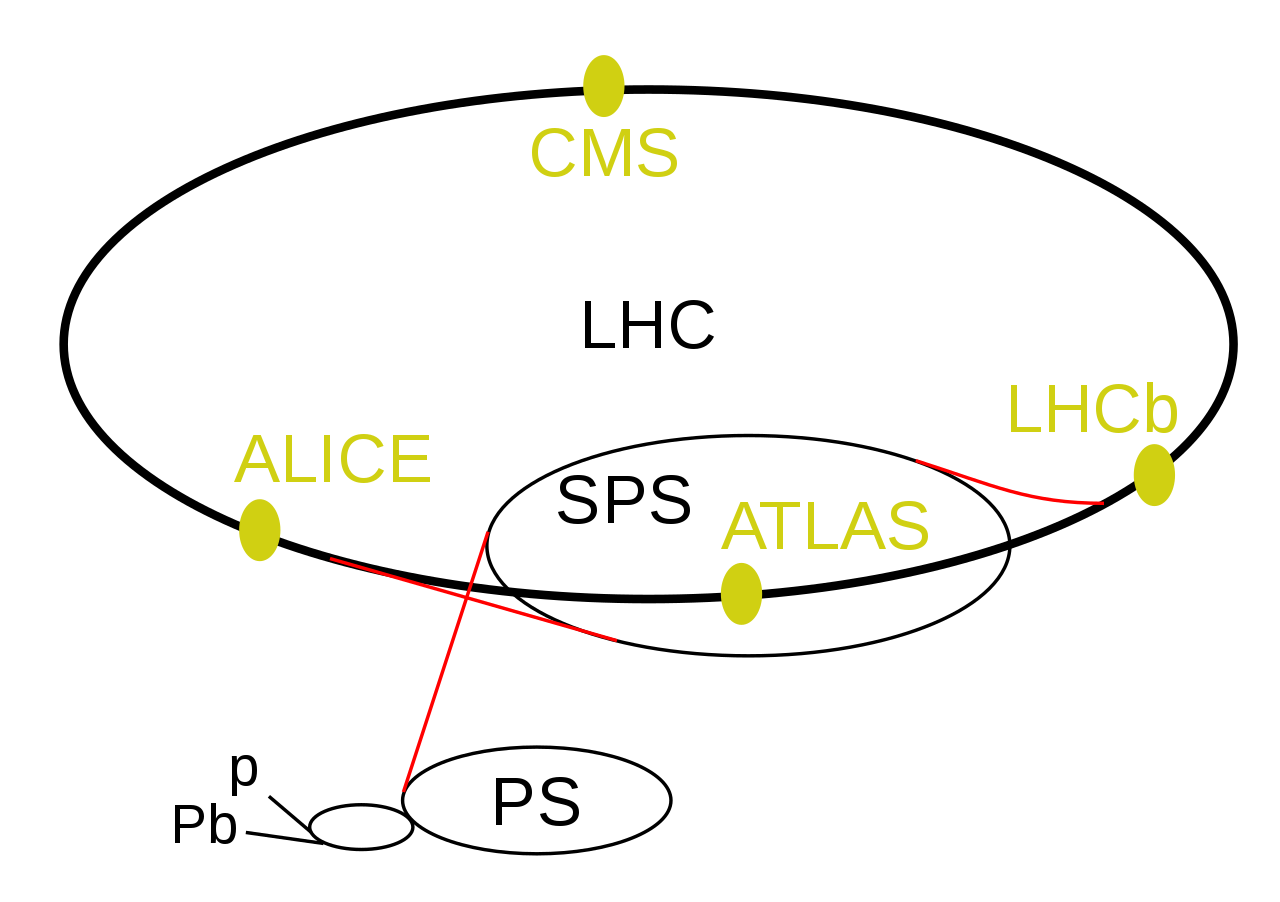
\includegraphics[scale=0.3]{MainContent/Figs/LHC.png}
	\caption{LHC experimental chain. The yellow dots represent the four main experiments. Retrieved from \cite{nobrega2013lhc}}
	\label{fig:LHC}
\end{figure}

\section{The CMS detector}

CMS is a general purpose detector used to reconstruct the decay products in proton and heavy-ion collisions at high energies. It can detect nearly any particle, especially muons, with high precision . CMS is located in a cavern about 100 m underground near Cessy, France. It has a cylindrical geometry, with a full length of 21.5 m and a diameter of 15 m. With a total weight of 12500 t, it is the heaviest detector in the LHC \cite{bragagnolo2021measurement, mejia2012medida}. CMS is operated by a large collaboration of members worldwide, consisting of over 4000 particle physicists, engineers, computer scientists, technicians, and students from around 200 institutes and universities from more than 40 countries \cite{cms_collab}. The University of Antioquia is one of the collaborating universities through the Phenomenology and Fundamental Interactions Group (GFIF) \cite{restrepo2019udea}.

The physical structure of the detector consists of a superconducting solenoid able to produce an internal, uniform 4T magnetic field. Inside the solenoid, there is a tracking system, also known as tracker, surrounded by a calorimetry system consisting of the Electromagnetic Calorimeter (ECAL) and the Hadron Calorimeter (HCAL). Outside the solenoid, there is a muon detector chamber. The detector is depicted schematically in Fig. \ref{fig:CMS_structure}.

\begin{figure}[htp!]
	\centering
	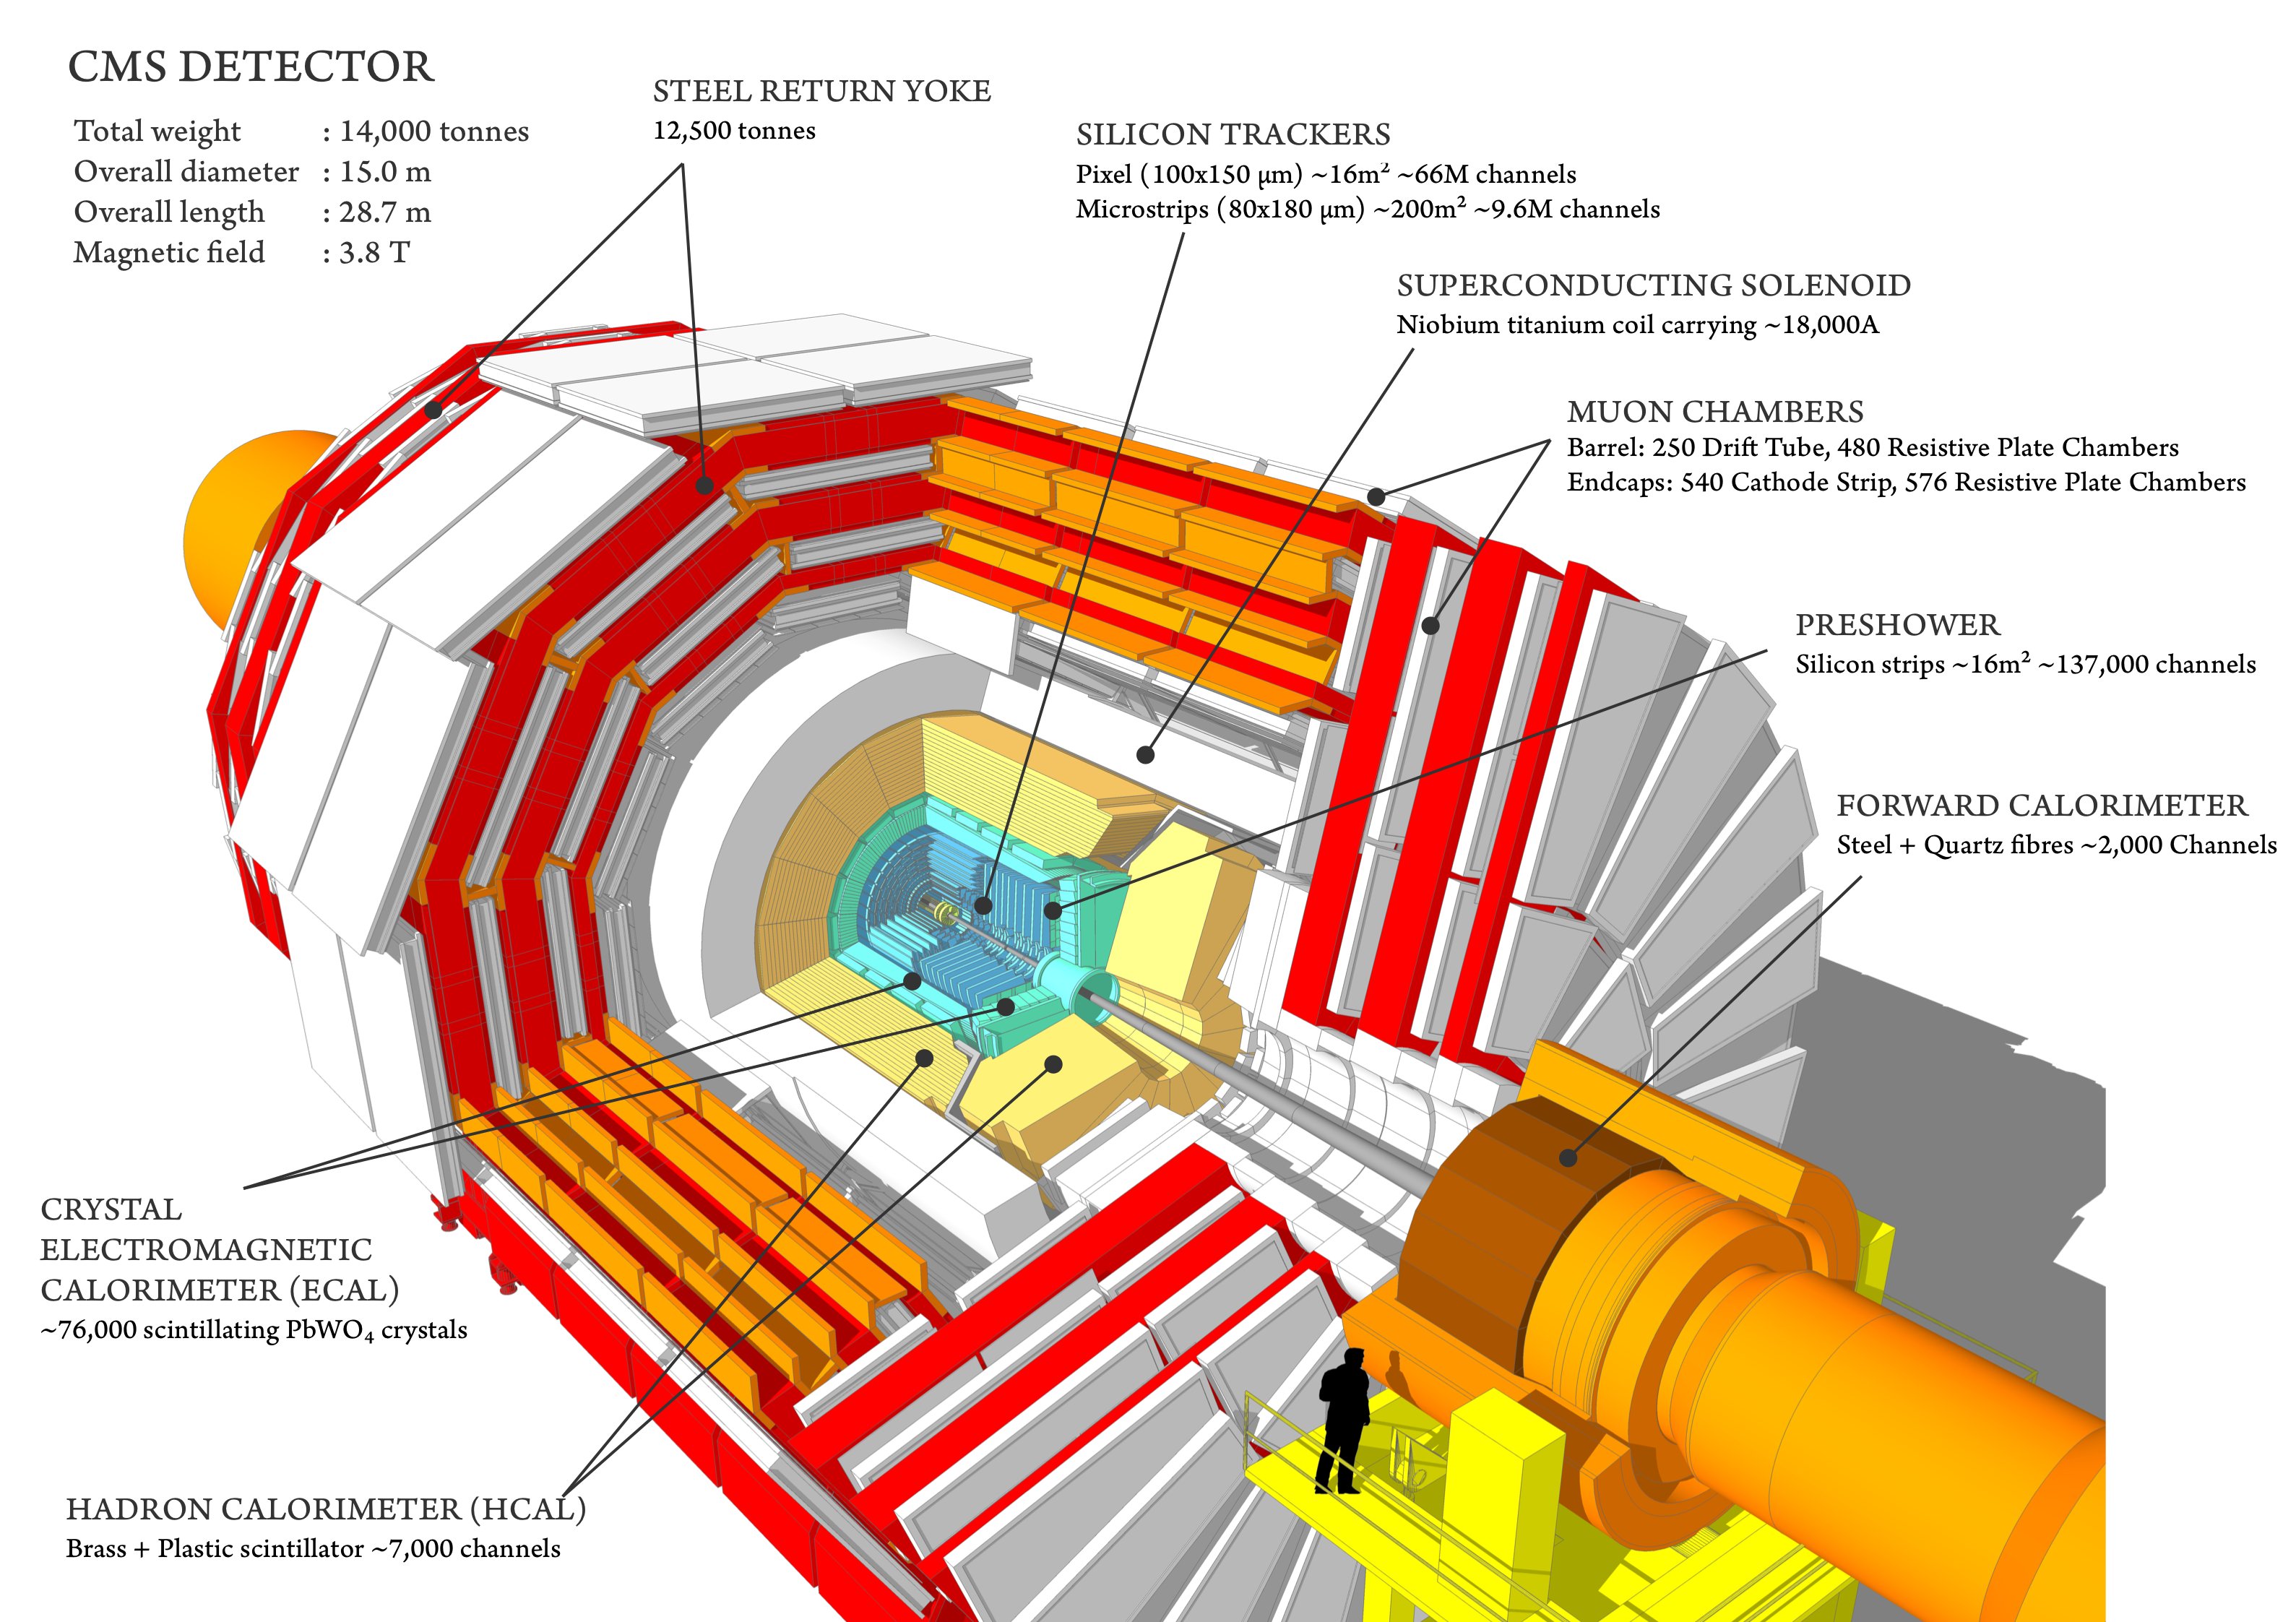
\includegraphics[scale=0.2]{MainContent/Figs/cms_structure.png}
	\caption{CMS internal structure with its main sub-systems. Retrieved from \cite{sanchez2020search}.}
	\label{fig:CMS_structure}
\end{figure}


Before delving deeper into the detector internal components, the coordinate system will be introduced in the following subsection.

\subsection{The coordinate system}
CMS uses a right-handed Cartesian coordinate system, with the origin at the center of the detector. The $x$-axis points towards the center of LHC, the $y$-axis points upwards, and the $z$-axis points in the counterclockwise direction of the beam. The $x-y$ plane is called the transverse plane and is perpendicular to the beam axis \cite{baron2018desarrollo, sanchez2020search, lechner2021measurement}. In this plane, two quantities can be defined: the azimuthal angle $\phi$ with respect to the x-axis and the particle transverse momentum, $p_T = \sqrt{p_x^2 + p_y^2}$. The polar angle $\theta$, on the other hand, is defined in the $z-y$ plane and measured from the $z$-axis. Fig. \ref{fig:cms_coordinate_system} illustrates the coordinate system.


\begin{figure}[htp!]
	\centering
	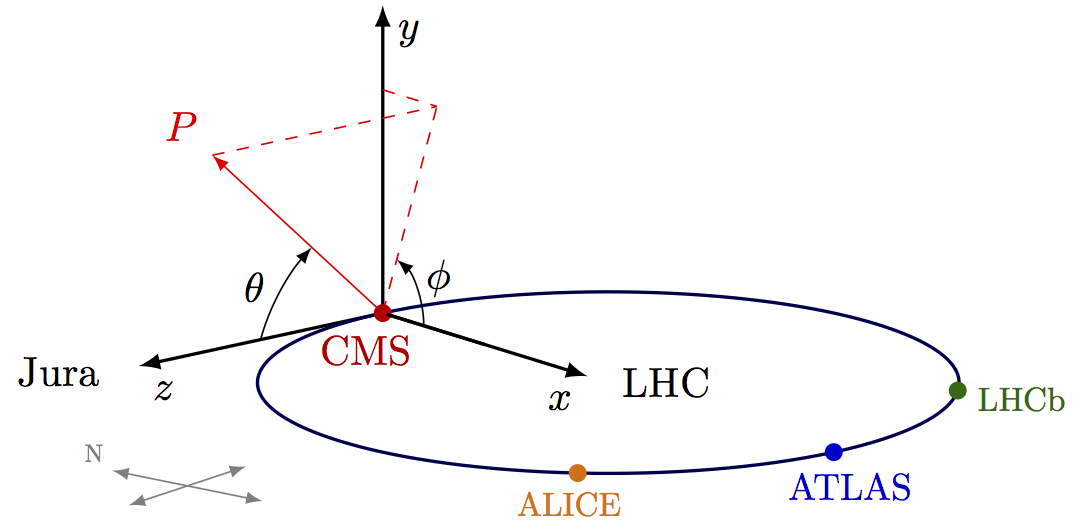
\includegraphics{MainContent/Figs/cms_coordinate_system.png}
	\caption{Illustration of the CMS coordinate system. Retrieved from \cite{bonanomi2021response}.}
	\label{fig:cms_coordinate_system}
\end{figure}

In this coordinate system, one can define two relativistic invariant quantities, the particle rapidity \cite{bonanomi2021response},

\begin{equation}
y = \frac{1}{2}\ln\left(\frac{E+p_z}{E-p_z}\right)
\end{equation}

and the pseudo-rapidity,

\begin{equation}
\eta = -\frac{1}{2}\ln\left(\frac{\theta}{2}\right)
\end{equation}

It is important to mention that the quantities $p_T$ and $\eta$ are considered in the results presented in Chapter 4.

\subsection{Superconducting Solenoid}
Located at its center, the superconducting solenoid is the key part of the CMS detector. The solenoid is made up of four layers of Nb-Ti coils and has a length of 12.5 m and a diameter of 6 m. It has a working temperature of 4.5K and it can produce a constant magnetic field inside of 4T, however, it is operated at 3.8T \cite{baron2018desarrollo, bragagnolo2021measurement}. A return yoke made of iron reduces the magnetic field outside the solenoid to about 2T. The magnet stores a total energy of 2.6 GJ \cite{fedi2016studies}. The magnetic field is used to bend the trajectory of the charged particles after the collision, thus allowing to measure their transversal momentum, $p_T$, and charge sign. The stronger the magnetic field, the larger the bending, and, hence, more precise measurements can be achieved \cite{sanchez2020search, presilla2021lepton}.
\subsection{The tracker}
The tracker, which is placed at the interaction point, is made up of two parts: a silicon pixel detector in the center and a silicon strip detector around it, both of which are made of superconducting technology but have different sizes and granularities \cite{sanchez2020search}. The pixel detector is very granular and consists of 66 million pixels spaced out over a radius of 10 cm, each pixel has a dimension of $100 \times 150 \ \mu \text{m}^2$. The strip detector contains 9.6 million of strips and has a length of 5.5 m and a diameter of 2.4 m \cite{fedi2016studies, danilov2020measurement}.

An electron-hole pair is formed in the material when a charged particle passes through the tracker. This generates an electrical signal, which is amplified and used to reconstruct the trajectory or tracks with a 98$\%$ percent efficiency and a precision of about $10 \ \mu$m in the range $|\eta| < 2.5$ \cite{baron2018desarrollo, di2020measurement}. The momentum of a particle is calculated using the trajectory. The tracker can also estimate the location of the secondary vertices where decays occur \cite{fedi2016studies}.
\subsection{Calorimetry system}
\label{cal_sys}
The calorimetry system of CMS is placed after the tracker. The reason for this is that the calorimetry system measures the energy of most particles by fully absorbing them, with the exception of neutrinos and neutrons \cite{bragagnolo2021measurement}. To achieve high accuracy in measurements, the system is divided into two sub-detectors, the ECAL and the HCAL, which are located between the tracker and the superconducting solenoid, with the ECAL in the innermost part \cite{presilla2021lepton}.

ECAL is a cylindrical detector that measures electron and photon energies and covers the pseudo-rapidity, $|\eta| < 3$. The ECAL is made up of approximately 76000 scintillating crystals of lead tungstate (PbWO$_4$) \cite{fedi2016studies, mejia2012medida}. This material was chosen because of its high density, short radiation length, and small Moliere radius \cite{danilov2020measurement}. It is also highly transparent due to its low concentration of oxygen, this is particularly useful because when photons and electrons pass close by, it scintillates with a light with an intensity proportional to the particle's energy. Photodetectors are used to measure this light \cite{di2020measurement, mejia2012medida}.

HCAL is a sampling and hermetic calorimeter with brass layers and plastic scintillators. It measures the energy of charged and neutral hadrons (protons, pions, kaons, neutrons, and so on) in the region $|\eta| < 5$ \cite{li2021measurements, muhammad2021measurement}. To accomplish this, when a particle passes close by, the brass layers produce a secondary hadron shower, and when these secondary hadrons interact with the scintillators, light is produced, which is then converted into an electric signal by hybrid photodiodes \cite{baron2018desarrollo, muhammad2021measurement}. HCAL can also measure the missing energy in the transverse plane, $E^{\text{miss}}_T$, which is primarily associated with weakly interacting particles such as neutrinos \cite{di2020measurement}.
\subsection{Muon detector}
CMS's name derives from one of its primary goals: muon detection. Muons are not absorbed by the calorimetry system due to their high penetrative power \cite{baron2018desarrollo, di2020measurement}. As a result, a system of muon detectors is installed in the CMS's outermost region. This system not only detects muons with high efficiency in the $\eta < 2.4$ region, but also measures their momenta, charge, and triggers when they are present \cite{sanchez2020search}. The muon detection method is based on gaseous technology: a charged particle ionizes a gas, causing drift currents that are later read out \cite{baron2018desarrollo, danilov2020measurement}.

The system is composed of three gaseous chambers: Drift Tubes (DT), Chatode Strip Chambers (CSC), and Resistive Plate Chambers (RPC). There are a total of 250 DTs located in the barrel region, covering $|\eta| < 1.2$. This has a nearly uniform magnetic field and low rate of particles. DTs can provide measurements in the $r\phi$ plane and the $z$-direction \cite{bragagnolo2021measurement, di2020measurement, muhammad2021measurement}. CSCs, on the other hand, are found in the endcap where there is a strong and non-uniform magnetic field. They cover the pseudorapidity $0.9 < |\eta| < 1.2$ and provide measurements of the hit coordinates. There are four layers, each with 540 CSCs chambers \cite{lechner2021measurement, muhammad2021measurement}. Finally, the triggering is carried out using approximately 1056 RPCs modules. They have a high time resolution of about 1 ns. Each module is made up of two parallel plates separated by a gas and operated in avalanche mode. RPCs are placed in both the barrel and endcaps and cover the region $|\eta| < 1.9$ \cite{di2020measurement, lechner2021measurement}.

At the time of writing this manuscript, 144 new muon detectors known as Gas Electron Multipliers (GEMs) had been installed in the CMS detector. Their main goal is to improve muon track identification and enable wider measurements in the forward region (the endcaps), where high doses of radiation are present. It is expected that 288 additional GEMs will be installed between 2023 and 2024 and 216 during between 2025 and 2027 \cite{cern2020ls2, cerngems}. The University of Antioquia is a member of the GEMs team, primarily assisting with hardware tests and software development \cite{cms25udea}. GEMs are not significant for this dissertation because the data used for analysis was collected in 2016.

\subsection{Trigger System}
\label{subsection:trig_sys}
In a single second, the amount of data derived from collision events is approximately $1$ PB (Petabyte) \cite{baron2018desarrollo}. With today's technology, it is impossible to save all the data generated during an experiment and not all of this data is actually relevant to the CMS program. As a result, a trigger system is used to reduce the amount of data that must be processed. The filtering process in the trigger is divided into two stages \cite{muhammad2021measurement}. The data is first passed through a hardware-based filter known as the Level-1 (L1) trigger, and then it is passed through the High-Level Trigger (HLT).

The L1 trigger must decide whether an event is to be disregarded in a short time interval of about 4 $\mu$s \cite{bragagnolo2021measurement}. To do so, it takes the input from the sub-detectors in the calorimetry and muon system and processes it with hardware-based algorithms that run in parallel on several FPGAs and ASICs \cite{muhammad2021measurement}. This information is roughly processed and reconstructed into simple physics objects such as muons, photons, electrons, jets, and their associated transverse energy. An algorithm called \verb|Global Trigger| decides if the event is then passed to the HLT trigger. The L1 trigger reduces the rate of event generation to around 100 KHz \cite{bragagnolo2021measurement, muhammad2021measurement}.

The HLT trigger uses a set of software-based algorithms that run in a farm of processors made up of commercial CPUs to process the events filtered by the L1 trigger \cite{bragagnolo2021measurement}. These algorithms are pre-selected based on the object of study. HLT uses data from all the detectors in the CMS to partially reconstruct the entire event \cite{bragagnolo2021measurement}. The decision time is approximately 200 ms, and HLT is capable of reducing the event production rate from 100KHz to approximately 200 Hz. This data can then be saved for offline use \cite{fedi2016studies, danilov2020measurement}.